\documentclass[a4paper,
listof=totoc,
bibliography=totoc
]{scrartcl}
%\documentclass[ngerman,12pt,onecolumn,twoside,titlepage,BCOR5mm,DIV12]{article}
\usepackage[a4paper,left=3cm,right=5cm,top=5cm,bottom=4cm,bindingoffset=5mm]{geometry}


\usepackage{mystyle}

%%%%%%%% BEGIN DOCUMENT %%%%%%%%%%%%%%%%%%%%%%%%%%%%%%%%%%%%%%%%%%%%%%%%%%%%%%
\begin{document}
\selectlanguage{ngerman}

% \documentclass[a4paper,10pt]{article}
% % Wenn Sie eine andere Dokumentenklasse benutzen, kann sich das Layout verschieben 
% %({scrreprt} verursacht beispielsweise einen ungewollten Seitenumbruch).
% % Sie können in diesem Fall versuchen, die Abstände (\vspace, siehe unten) anzupassen 
% % oder Sie compilieren das Titelblatt einzeln mit der Dokumentenklasse "`article"'.
% \usepackage{graphicx}
% \usepackage{float}
% \usepackage[T1]{fontenc}
% 
% \begin{document}
\thispagestyle{empty}

\hspace{20cm}
\vspace{-2cm}

\begin{center}
  %\vspace{0.5 cm}
  \huge{\bf Titel der Arbeit} \\ % Hier fuegen Sie den Titel Ihrer Arbeit ein.
  \vspace{1cm}
  \LARGE  Bachelorarbeit \\ % Geben Sie anstelle der Punkte an, ob es sich um eine
                % Diplomarbeit, eine Masterarbeit oder eine Bachelorarbeit handelt.
  \vspace{0.3cm}
  \large Abschlussarbeit zur Erlangung des akademischen Grades Bachelor of Science (B.Sc.) \\
an der Hochschule für Technik und Wirtschaft Berlin \\ % Bitte tragen Sie hier anstelle der Punkte ein:
         % Diplominformatiker(in),
         % Bachelor of Arts (B. A.),
         % Bachelor of Science (B. Sc.),
         % Master of Education (M. Ed.) oder
         % Master of Science (M. Sc.).
  \vspace{1cm}
  {\large
    %\bf{
      \scshape
      %Humboldt-Universit\"at zu Berlin \\
      Fachbereich Informatik, Kommunikation und Wirtschaft \\
      Studiengang Informatik und Wirtschaft\\
    %}
  } 
  % \normalfont
\end{center}
\vspace {0.5 cm}% gegebenenfalls kleiner, falls der Titel der Arbeit sehr lang sein sollte
%{3.2 cm} bei Verwendung von scrreprt, gegebenenfalls kleiner, falls der Titel der Arbeit sehr lang sein sollte
{\large
  \begin{tabular}{llll}
    eingereicht von:    & Vorname Name && \\ % Bitte Vor- und Nachnamen anstelle der Punkte eintragen.
    Matrikelnummer:     & 123456          &&
    %geboren am:         & 02.11.1980 && \\
    %in:                 & Berlin && \\
    \cr&\\
    Gutachter/Innen: & Prof. Dr. xy && \\
		      & yz && \\% Bitte Namen der Gutachter(innen) anstelle der Punkte eintragen
				 % bei zwei männlichen Gutachtern kann das (innen) weggestrichen werden
    &&&\\
    eingereicht am:     & \dots\dots  \hspace{3cm} verteidigt am: & \dots\dots \\ % Bitte lassen Sie
                                    % diese beiden Felder leer.
                                    % Loeschen Sie ggf. das letzte Feld, wenn
                                    % Sie Ihre Arbeit laut Pruefungsordnung nicht
                                    % verteidigen muessen.
  \end{tabular}
}
\vspace{0.3 cm}
\begin{figure}[H] 
  \begin{center}
    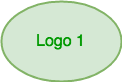
\includegraphics[width=4 cm]{img/logo1}
    \hspace{2cm}
    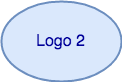
\includegraphics[width=4 cm]{img/logo2}
  \end{center}
\end{figure}
% \end{document}


%%%%%% ALTES TITELBLATT:
% %%%%%%%% TITLE %%%%%%%%%%%%%%%%%%%%%%%%%%%%%%%%%%%%%%%%%%%%%%%%%%%%%%%%%%%%%%%%%
% \begin{minipage}{17cm}
% %\begin{titlepage}
% \thispagestyle{empty}
% \begin{center} 
% \LARGE{ \vspace{2ex} Diplomarbeit}\\[4ex] 
% \huge{Rankingverfahren für Dokumentensuche basierend auf Ontologie-Relationen} \\[4ex]
% \large{ eingereicht von: Benjamin Großmann}\\[4ex]
% \large{ Berlin, den \dategerman \today}\\[8ex]
% 
%   \normalsize{
%   \psfig{figure=Bilder/husiegel_sw_klein,height=16ex}\\
%   Mathematisch-Naturwissenschaftliche \\Fakult\"at II\\Institut f\"ur Informatik\\[4ex]
%   }
%   \large{Betreuer:\\[1ex]
% %	Dr. Christian Herta, neofonie GmbH \\ [1ex]
% %	Prof. Dr. Hans-Dieter Burkhard, Humboldt-Universität zu Berlin, Lehrstuhl Künstliche Intelligenz
% 	}
% 	
% \end{center}
% \end{minipage}
%\newpage

%\include{tex/zusammenfassung}

%%%%%%%% TABLE OF CONTENT %%%%%%%%%%%%%%%%%%%%%%%%%%%%%%%%%%%%%%%%%%%%%%%%%%%%%%
\setcounter{tocdepth}{-1}
\section*{Eidesstattliche Versicherung}
Ich versichere hiermit, dass ich die vorliegende Bachelorarbeit selbstständig und ohne fremde Hilfe angefertigt und keine andere als die angegebene Literatur benutzt habe. Alle von anderen Autoren wörtlich übernommenen Stellen wie auch die sich an die Gedankengänge anderer Autoren eng anlehnenden Ausführungen meiner Arbeit sind besonders gekennzeichnet. Diese Arbeit wurde bisher in gleicher oder ähnlicher Form keiner anderen Prüfungsbehörde vorgelegt und auch nicht veröffentlicht.\\
Berlin, den {\today} 
\\\\
Vorname Name 

\pagebreak
\section*{Sperrvermerk}

Die vorliegende Arbeit enthält vertrauliche Daten der **Firma**. Die Weitergabe des Inhalts der Arbeit im Ganzen oder in Teilen sowie das Anfertigen von Kopien oder Abschriften -- auch in digitaler Form -- sind grundsätzlich untersagt. Ausnahmen bedürfen der schriftlichen Genehmigung der **Firma**.\\
Berlin, den {\today} 
\\\\
Vorname Name 
\pagebreak

\setcounter{tocdepth}{2}
\tableofcontents
\pagebreak

%\include{tex/erklaerung}

\section{Einleitung}
\label{chapter:Einleitung}

Die ist die Einleitung mit einer Aufzählung: 

\begin{enumerate}
\item Dies ist eine Vorlage für Bachelorarbeiten
\item Latex :-)
\end{enumerate}

Für weiteres siehe Abbildung \ref{fig:beispiel_abbildung}. 

\begin{figure}[htb]
\centering
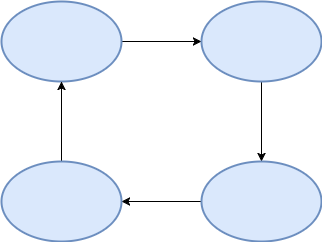
\includegraphics[width=\linewidth]{img/beispiel} 
\caption{Eine Abbildung }
\label{fig:beispiel_abbildung}
\end{figure}

\subsection{Zielsetzung}
\label{chapter:Zielsetzung}
Ziel dieser Arbeit ist es, einen Service mit einer Schnittstelle für JSON zu implementieren..... Für weiteres siehe lies den Abschnit \ref{chapter:microservice}.
\section{Grundlagen}
\label{chapter:grundlagen}

\subsection{Microservices} 
\label{chapter:microservices}
Bei Microservices handelt es sich um ein Architekturmuster zur Modularisierung von Software mit dem Ziel einer besseren Skalierbarkeit. Um die Modularisierung sicherzustellen, werden die Module als unabhängige Services implementiert. Diese Services kommunizieren über das Netzwerk über klar definierte Schnittstellen miteinander.

Charakteristisch für Microservices ist die Eigenständigkeit: Jeder Service läuft als eigener Prozess und lässt sich einzeln installieren und starten.
\begin{quote}
 Die Idee der Microservices "`[...] basiert auf der UNIX-Philosophie. Sie lässt sich auf drei Aspekte reduzieren:
\begin{itemize}
 \item Ein Programm soll nur eine Aufgabe erledigen, und das soll es gut machen.
 \item Programme sollen zusammenarbeiten können.
 \item Nutze eine universelle Schnittstelle. In UNIX sind das Textströme."'
\end{itemize}
\cite[2]{wolff_microservices:_2015}
\end{quote}

Für den Begriff Microservices gibt es keine feste Definition. Wolff nennt folgende Kriterien: 
\begin{itemize}
 \item Modularisierungskonzept zum Aufteilen großer Software-Systeme
 \item Unabhängiges Deployment
 \item Verwendung verschiedener Technologien (z.B. Programmiersprachen) möglich
 \item Separate Datenhaltung, beispielsweise Nutzung separater Datenbanksysteme oder konsequente Trennung der Datennutzung innerhalb desselben Datenbanksystems
 \item Eigenständige Prozesse oder virtuelle Maschinen
 \item Kommunikation über das Netzwerk
\end{itemize}
\cite[2]{wolff_microservices:_2015}

Auffällig ist, dass bei dieser Definition die Größe des Services nicht betrachtet wird, obwohl der Name vermuten lässt, dass es sich um einen kleinen Service handelt. 
Es gibt verschiedene Faktoren, die die ideale Größe eines Microservices beeinflussen. Modularisierung ist ein Ansatz, um die Komplexität der Software gering zu halten. Kleine Services sind weniger komplex, dadurch leichter zu verstehen und somit leichter zu ändern. Jedoch muss man dabei bedenken, dass Microservices in eigenständigen Prozessen laufen, so dass eine verteilte Kommunikation zwischen diesen nötig wird. Diese Kommunikation benötigt zusätzliche Zeit und ist potenziell fehleranfälliger im Vergleich zu einer Kommunikation innerhalb der Anwendung. Beim Design von Microservices gilt es, beide Seiten zu beachten und eine gute Größe zu wählen. Wolff rät zur Entwicklung größerer Services. \cite[31ff.]{wolff_microservices:_2015} 
Eugene Kalenkovich kritisiert dagegen schon den Begriff Microservices:
\begin{quote}"`All this hype about microservices makes me sad. And not about the concept, but about the name. As I wrote before, “micro” in “microservices” means absolutely nothing. What is worse, it confuses everybody. Again and again I see people focusing on “micro” and falling into nanoservices trap."' \end{quote} \cite{kalenkovich_can_2014}

Auch Roland Kuhn findet den Begriff aufgrund seiner Mehrdeutigkeit unpassend und schlägt stattdessen den Begriff Uniservice vor. \cite{kuhn_microservice_2014}
Im Diskurs über Servicearchitekturen findet man ebenfalls die Begriffe "`decoupled services"' und "`SOA done right"'. \cite{white_microservices_2015} 


\section{Anforderungsanalyse}

\begin{enumerate}
    \item eine Anforderung.....
    \item noch eine Anforderung....
\end{enumerate}

\subsection{Nichtfunktionale Anforderungen}
\begin{enumerate}
    \item Die Anfragen an den xx werden so effizient wie möglich gestaltet. 
    \item Der Service muss skalierbar sein. Bei einem Microservice bedeutet Skalierbarkeit, dass weitere Instanzen nach Bedarf gestartet werden können.
    \item Die Richtlinien zur Codequalität werden eingehalten. 
\end{enumerate}

\section{Methoden}
\label{chapter:methoden}

\subsection{Programmiertechniken}
.......

\subsubsection{Logging mit MDC}
log4j \footnote{\url{https://logging.apache.org/log4j}} ist ein Logging-Framework für Java. Es bietet mit dem Mapped Diagnostic Context, im Weiteren mit MDC abgekürzt, die Möglichkeit, Informationen zu loggen, ohne diese in die ausführende Methode hineinzugeben. Man kann beispielsweise zu Beginn einer Anfrage eine ID vergeben und diese als Feld an alle Log-Nachrichten bei der Verarbeitung der Anfrage einfügen, wie das Code-Beispiel in Listing \ref{lst:JavaMdc} zeigt.

\begin{lstlisting}[
  caption=Setzen eines Feldes für Log-Nachrichten mit MDC,
  label=lst:JavaMdc,
  language=Java,
  float=htb]
import org.apache.log4j.MDC;
public class LogExample {
    public void startRequest(String requestId) {
        MDC.put("requestId", requestId);    
        // process request....
        MDC.remove("requestId);
    }
\end{lstlisting}

Mit \textit{MDC.put} wird der Wert für das angegebene Feld, in diesem Beispiel \mbox{\textit{requestId}}, gespeichert und solange in allen Log-Nachrichten ausgegeben, bis es mit \textit{MDC.remove} wieder gelöscht wird. 
 
\section{Umsetzung}
\label{chapter:umsetzung}

Die \textbf{Status} sind in \textit{Tabelle} \ref{tab:beispiel} beschrieben. 

\begin{table}[!ht]
\centering
\begin{tabular}{l p{8cm} } 
  \toprule
\textbf{Status} & \textbf{Beschreibung} \\ \midrule
  \texttt{OK} & Das Angebot wurde korrekt verarbeitet. \\
  \texttt{WARNING} & Das Angebot konnte verarbeitet werden, es wurden aber nicht alle Felder übernommen. \\
  \texttt{NOT\_FOUND} & Das Angebot konnte nicht gelöscht werden, da es nicht existiert. \\
  \texttt{FAIL\_TEMPORARILY} & Das Angebot konnte nicht importiert werden, es wird eine Wiederholung empfohlen. \\
\bottomrule
\end{tabular} 
\caption{Beispieltabelle}
\label{tab:beispiel}
\end{table}


\section{Auswertung und Ausblick}
\label{chapter:auswertung}


\setcounter{secnumdepth}{0}
\section{Abkürzungsverzeichnis}

\begin{tabular}{ll}
API             & Application Programming Interface \\
HTTP            & Hypertext Transfer Protocol \\
JSON            & JavaScript Object Notation \\
MDC             & Mapped Diagnostic Context \\
OM              & OfferManager \\
OM-Publisher    & Offermanager-Publisher \\
PWS             & PartnerWebservice \\
SQALE           & Software Quality Assessment based on Lifecycle Expectations\\
REST            & Representional State Transfer \\
RFC             & Request for Comments \\
UUID            & Universally Unique Identifier \\
URI             & Uniform Resource Identifier \\ 
\end{tabular}


 
\pagebreak
\listoffigures
\listoftables
\lstlistoflistings
\pagebreak


%%%%%%%% REFERENZEN %%%%%%%%%%%%%%%%%%%%%%%%%%%%%%%%%%%%%%%%%%%%%%%%%%%%%%%%%%%%

%\nocite*

\bibliographystyle{plainnat} %abbrv
\raggedright{
\bibliography{Literatur/literatur.bib}}
\pagebreak
\section{Anhang}



\end{document}
